\chapter{Fitting the Models}

\section{Linear Regression}

Linear regressions were fit, with and without regularization. Of the 192 models fit, 48 models did not use regularization and the other 144 were split amongst ridge, lasso, and elastic net. The models were combinations of granularity (daily or monthly), type of predictors (factors or themes), data time frame (2001-2024 or 2016-2024), market returns being predicted (U.S. or China), origin of the predictors used (U.S. data, China data, or both).

As suggested by the literature, the $R^2$ value is computed as a measure of explainability. I've also computed the Adjusted-$R^2$ value as an extra measure that considers the number of variables used. Adjusted-$R^2$ is used to penalize using more predictors, which can help in finding models that were most efficient.

\subsection{Assumptions}

The main assumptions on the data in a regression are the lack of multicollinearity, homoskedasticity, and normality and independence in the errors. 

The data has so far been standardized. Testing for multicollinearity revealed one near-perfect correlation in the daily factors datasets and in the monthly factors dataset, and no near-perfect collinearity in the themes datasets. The correlation pair for both was turnover\_126d and zero\_trades\_126d, both of which were removed from the datasets for the U.S. and China.

For each of the models trained, residual and Q-Q plots are assessed. Trends are described below.

\subsection{Without Regularization}

The linear regression without regularization results are shown in Table~\ref{tab:usa_market_regression_summary} and Table~\ref{tab:chn_market_regression_summary}, separated by the market being replicated. Note that six models returned an $R^2$ of 1 and an Adjusted-$R^2$ of 0. Those cases resulted from models in which the number of rows in the data was lower than the number of predictors. This was the case when estimating 2016-2024 monthly data using facts; recall that there are about 140 factors remaining in the data for each country and there are about 114 months in the analyzed time frame. The Adjusted-$R^2$ of 0 was a safeguard in my code to prevent an erroneous calculation.

Analyzing the models that predicted U.S. returns using the daily data, we note that there was no scenario in which using Chinese economic data alone had an $R^2>0.10$. Using economic data from both countries also produced negligible effects on the $R^2$ value, as compared to using only U.S. economic data. Analyzing the models that predicted Chinese returns using the daily data, we note that the best performing model using only U.S. economic data had $R^2=0.19$. Using U.S. economic data along with Chinese economic data seems to have bigger impacts; in the factors model on 2016-2024 data, it increased the $R^2$ from 0.5948 to 0.6728 (see Table~\ref{tab:table1}).

\begin{table}[htbp]
\centering
\caption{Chinese Returns Regression using U.S. and Chinese Factors}
\label{tab:table1}
\begin{tabular}{@{}llllrr@{}}
\toprule
Time Period & Granularity & Predictors & Adjusted $R^2$ & $R^2$ \\ \midrule
2016--2024 & Daily   &  usa\_factors  & 0.0815  & 0.1910 \\
2016--2024 & Daily   &  chn\_factors  & 0.5599  & 0.5948 \\
2016--2024 & Daily   &  both\_factors & 0.5918  & 0.6728 \\ \bottomrule
\end{tabular}
\end{table}

The fitted models typically had four types of Q-Q and residual plots. In the first case, the residual plots (see Figure~\ref{fig:label25} for an example) seemed normally distributed and the Q-Q plots (see Figure~\ref{fig:label29}) displayed some deviations towards the extremes in the data. 

In the second case, the residual plots (see Figure~\ref{fig:label26} for an example) seemed Normally distributed, but there were clear linear boundaries in the residuals, and the Q-Q plot (see Figure~\ref{fig:label30}) displayed some greater deviations towards the ends of the data. The residual plots' trends suggest that there might be an underlying constraint or structure in the data that isn't fully captured by the model, potentially as a result of a transformation.

\begin{figure}[htbp]
\begin{center}
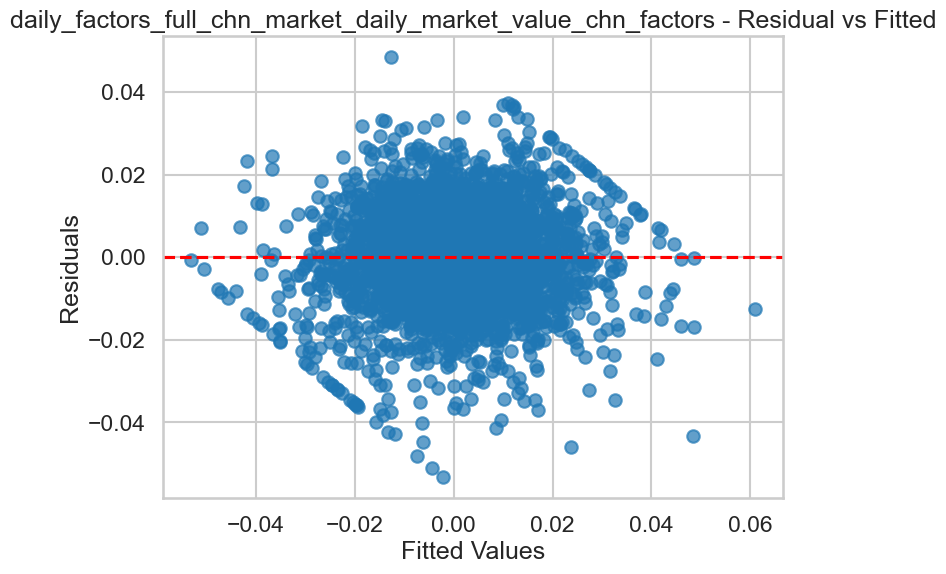
\includegraphics[width=3.5in]{figures/regression/residual2.png}
\caption{Case 2: Residual Plot}
\label{fig:label26}
\end{center}
\end{figure}

In the third case, the residual plots (see Figure~\ref{fig:label27} for an example) showed clear trends in the data and the Q-Q plot (see Figure~\ref{fig:label31}) only showed issues on the most extreme data points. The residual plots' trends suggest that the linear assumption in the data might be very limiting, and that the underlying data might not follow the necessary structure.

\begin{figure}[htbp]
\begin{center}
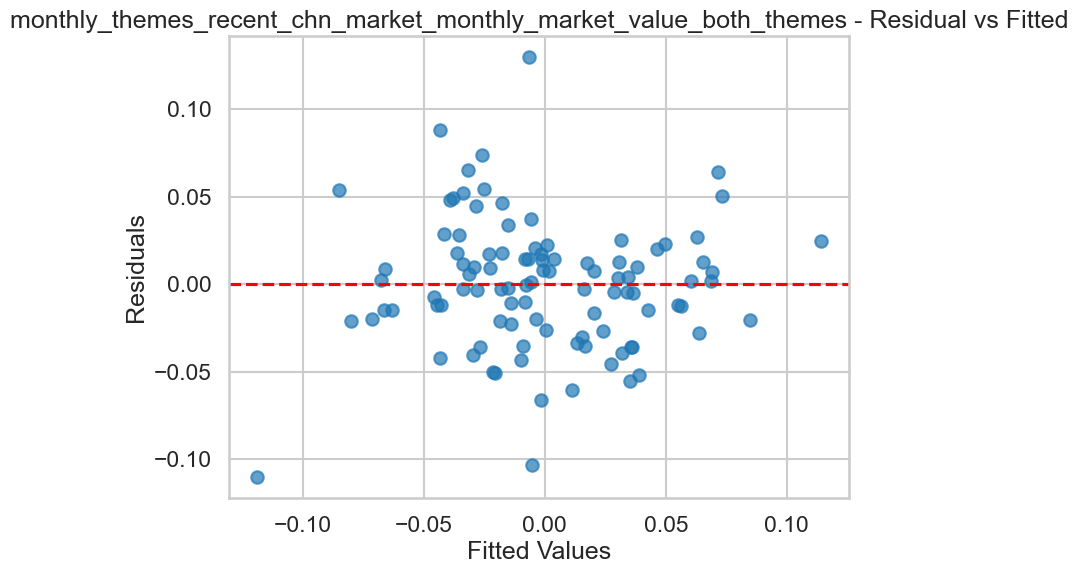
\includegraphics[width=3.5in]{figures/regression/residual3.png}
\caption{Case 3: Residual Plot}
\label{fig:label27}
\end{center}
\end{figure}

In the fourth case, the residual plots (see Figure~\ref{fig:label28} for an example) showed signs of increasing variance over time and the Q-Q plot (see Figure~\ref{fig:label32}) displayed some deviations towards the ends of the data. The residual plots' trends suggest heteroscedasticity in the data, which can impact the reliability of the model. The Q-Q plot suggests that this is mainly at the extreme ends of the data.

\begin{figure}[htbp]
\begin{center}
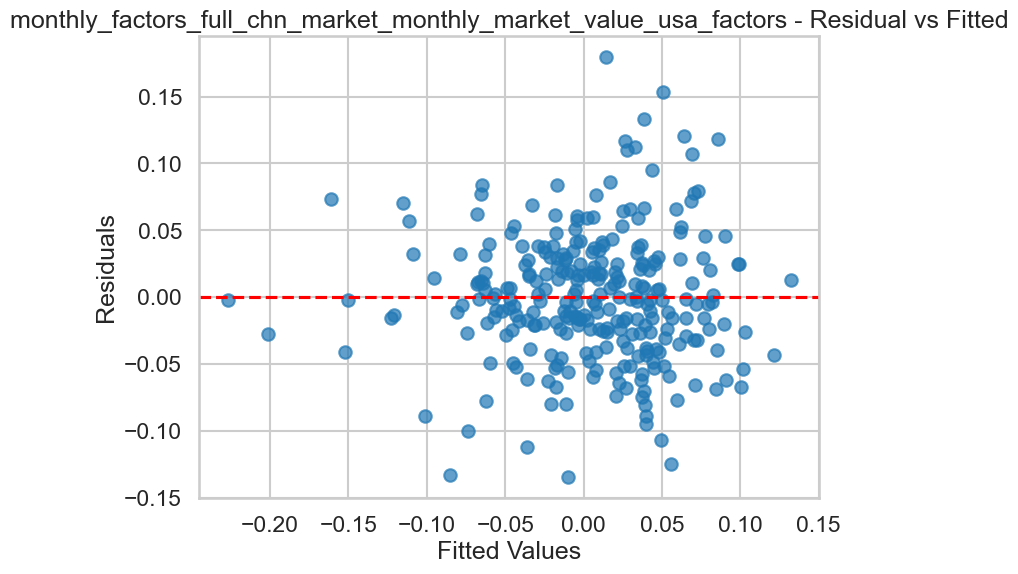
\includegraphics[width=3.5in]{figures/regression/residual4.png}
\caption{Case 4: Residual Plot}
\label{fig:label28}
\end{center}
\end{figure}

These plots suggest that the linear regressions are not capturing the full relationship between the data. Before moving onto models that do not assume linearity, let's assess regressions with regularization.

\subsection{With Regularization}

Using sklearn, I fit a total of 144 models using either ridge, lasso, or elastic net regularization. The standardscaler was used once again to ensure that everything is standardized; note that while this process might be redundant, it does not impact the data. Grid search cross-validation is used to tune the hyperparameters for each regression based on minimizing the MSE. The TimeSeriesSplit method was used to account for the temporal structure of the data, ensuring that the training and validation data split is somewhat uniform across time. 

The best model of the three regularization methods was used. Of the 48 models, Ridge was the best model by $R^2$ for 45; Lasso was the best for two and Elastic Net was the best for one. Similar to the previous regression section, the results are split between those predicting U.S. returns (see Table~\ref{tab:usa_market_regularized_regression_summary}) and those predicting Chinese returns (see Table~\ref{tab:chn_market_regularized_regression_summary}).

We note no significant gain was added to the $R^2$ value when predicting U.S. returns when Chinese predictors were also included. When Chinese predictors were used to predict U.S. returns, they had at most an $R^2$ of 0.1341; this was also a scenario in which adding the Chinese predictors to the U.S. predictors actually decreased the $R^2$ of the general model.

\begin{table}[htbp]
\centering
\caption{Best Regularized Model for U.S. Returns}
\label{tab:table2}
\begin{tabular}{@{}llllrr@{}}
\toprule
Time Period & Granularity & Predictors     & Technique & Adjusted $R^2$ & $R^2$ \\ \midrule
2001--2024  & Daily       & both\_factors  & Ridge          & 0.7385         & 0.7510 \\
2001--2024  & Daily       & chn\_factors   & Ridge          & 0.0036         & 0.0272 \\
2001--2024  & Daily       & usa\_factors   & Ridge          & 0.7378         & 0.7441 \\ \bottomrule
\end{tabular}
\end{table}

We see similar trends in the Chinese market regressions, in which the highest $R^2$ using only U.S. predictors was 0.2210. This was also a scenario in which adding the U.S. predictors to the Chinese predictors decreased the $R^2$ of the model. Generally, we also note lower $R^2$ values in the models than in those predicting U.S. returns.

\begin{table}[htbp]
\centering
\caption{Best Regularized Model for Chinese Returns}
\label{tab:table3}
\begin{tabular}{@{}llllrr@{}}
\toprule
Time Period & Granularity & Predictors     & Technique & Adjusted $R^2$ & $R^2$ \\ \midrule
2016--2024  & Daily       & both\_factors  & Lasso          & 0.4712         & 0.5761 \\
2016--2024  & Daily       & chn\_factors   & Ridge          & 0.5162         & 0.5545 \\
2016--2024  & Daily       & usa\_factors   & Ridge          & -0.0105        & 0.1100 \\ \bottomrule
\end{tabular}
\end{table}

A few trends were exhibited in the regularized models. There were trends similar to Case 1 from above, in which the residual plot seemed scattered with normality holding for most of the data, tapering off towards the ends of the data. There were many cases similar to Case 2, in which the residual plot had some linear boundaries. Interestingly, those were sometimes accompanied with far worse Q-Q plots (see Figure~\ref{fig:label33})) in which most of the data was not normal and the outliers were very extreme. This suggests that the residuals are far from a normal distribution, showing violations in the assumption of a normally distributed error term.

\begin{figure}[htbp]
\begin{center}
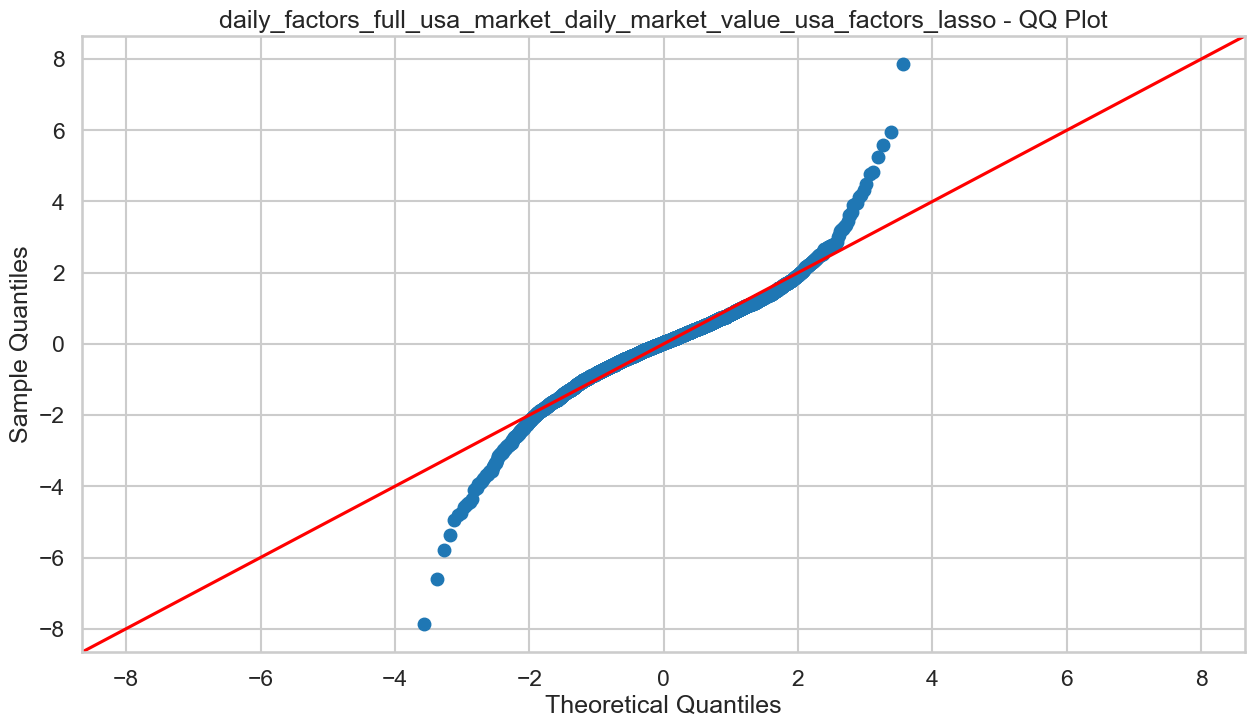
\includegraphics[width=3.5in]{figures/regression/qq6.png}
\caption{Curved Q-Q Plot}
\label{fig:label33}
\end{center}
\end{figure}

One model's residual plot exhibited linear constraints from all four edges, forming an outlining square (see Figure~\ref{fig:label34})). This was associated with curved Q-Q plots that generally followed the theoretical quantiles (see Figure~\ref{fig:label35}).

\begin{figure}[htbp]
\begin{center}
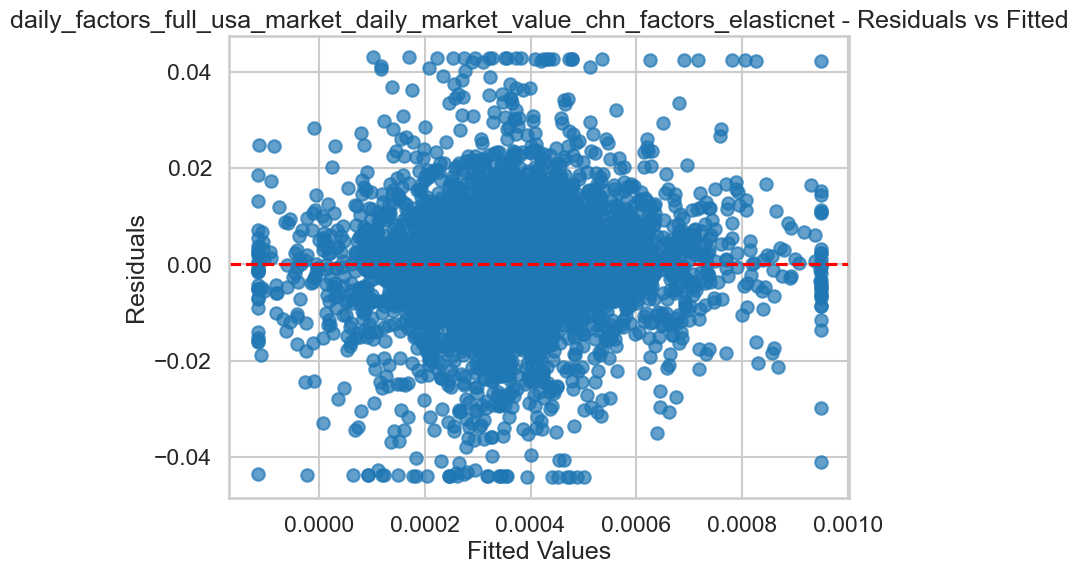
\includegraphics[width=3.5in]{figures/regression/residual5.png}
\caption{Square Outline in Residual Plot}
\label{fig:label34}
\end{center}
\end{figure}

These plots motivate the next attempts with Sparse Additive Models (SpAMs), which do not assume a linear relationship between the predictors and the returns. Note that it does assume an additive effect, not accounting for interactions between the themes. 

\section{Sparse Additive Model}

Using the pyGAM package, I ran 24 SpAMs on the theme data. Each predictor is assigned a spline term with 10 splines. The additive model is the sum of the spline terms. It is fitted using grid search to find the optimal parameters.

Note that I decided to run the SpAMs on only the theme data as one of the main advantage of a SpAM is to determine the marginal relationship between a predictor and the outcome variables. The factors are too granular to provide a strong economic interpretation unless there is a specific set of factors being investigated.

The $R^2$ and Adjusted-$R^2$ measures for the SpAM models for U.S. market returns are shown in Table~\ref{tab:spam_usa_market}. We note that the Chinese themes alone were able to explain at most 6.33\% of the variation in the U.S. market returns, yet again hinting at a lack of signaling from the Chinese to U.S. markets. We note that the model fit on 2016-2024 data using both themes yielded an $R^2$ of 0.9999; while SpAM does integrate some form of regularization, this is likely a case of overfitting. 


\begin{table}[htbp]
\centering
\caption{SpAM Regressions Predicting U.S. Market Returns}
\label{tab:spam_usa_market}
\begin{tabular}{@{}llllrr@{}}
\toprule
Time Period & Granularity & Predictors     & Adjusted $R^2$ & $R^2$ \\ \midrule
2001--2024  & Daily       & both\_themes   & 0.5949          & 0.6032 \\
2001--2024  & Daily       & chn\_themes    & 0.0078          & 0.0120 \\
2001--2024  & Daily       & usa\_themes    & 0.5970          & 0.6022 \\
2016--2024  & Daily       & both\_themes   & 0.5507          & 0.5687 \\
2016--2024  & Daily       & chn\_themes    & 0.0123          & 0.0222 \\
2016--2024  & Daily       & usa\_themes    & 0.5579          & 0.5714 \\
2001--2024  & Monthly     & both\_themes   & 0.6140          & 0.6538 \\
2001--2024  & Monthly     & chn\_themes    & 0.0100          & 0.0633 \\
2001--2024  & Monthly     & usa\_themes    & 0.6127          & 0.6359 \\
2016--2024  & Monthly     & both\_themes   & 0          & 0.9999 \\
2016--2024  & Monthly     & chn\_themes    & 0.0196          & 0.0459 \\
2016--2024  & Monthly     & usa\_themes    & 0.4725          & 0.5723 \\ \bottomrule
\end{tabular}
\end{table}

Observing some of the partial effects of the themes in the model support our speculations of the model being overfit. This is frequently detected by very wavy curves that do not follow economic intuition. The marginal effect for Chinese theme for debt issuance, seen in Figure~\ref{fig:label38}, is very wavy in a way that does not match economic intuition. You would expect that any relationship between Chinese debt issuance to not be so wavy; according to this model, changing debt issuance by -1.2, -0.3, 0.3, 0.8, and 1.4 all have the same zero-effect.

\begin{figure}[htbp]
\begin{center}
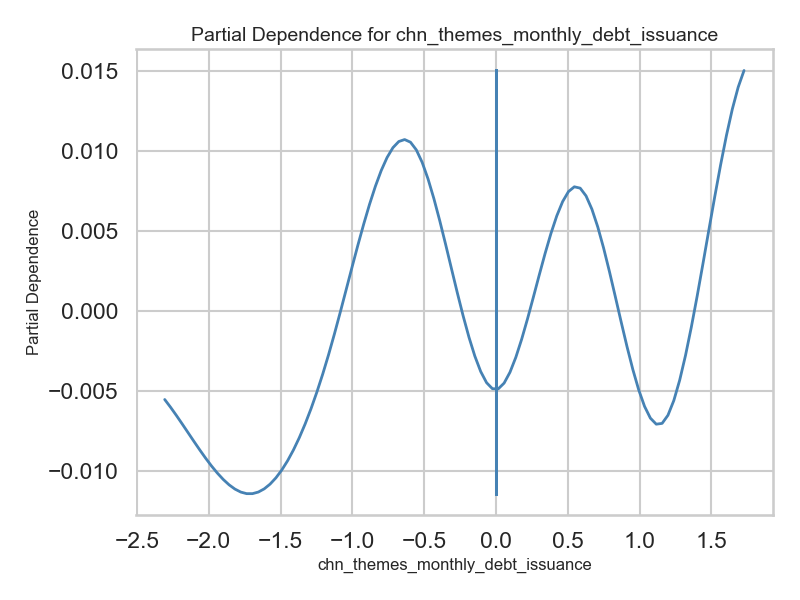
\includegraphics[width=3.5in]{figures/SpAM/overfit/partial_chn_themes_monthly_debt_issuance.png}
\caption{Partial Dependence of Chinese Debt Issuance on Overfit SpAM Model}
\label{fig:label38}
\end{center}
\end{figure}

The best model for U.S. market returns by $R^2$ is thus the model trained on 2001 to 2024 using U.S. and Chinese themes, with $R^2=0.6538$. Most of the partial dependence plots of the themes follow a linear structure, with the exception of Chinese Value and U.S. Momentum. 

Chinese value (see Figure~\ref{fig:label39}) is shown to have a strongly curved decreasing relationship, in which negative changes in Chinese Value estimates are estimated to be related to raises in the U.S. market. Recall that Value measures how many stocks are trading at lower prices relative to their values of fundamental measures. As stocks in China become overvalued, it makes sense that investors might shift their portfolios to U.S. stocks. On the other hand, increases in Chinese Value are related to diminishing effects on the U.S. market; this makes sense when you consider how much easier it has historically been to invest in the U.S. market as a foreigner than in the Chinese market. Still, we see a negative impact when Chinese value is increased, which aligns with economic intuition.

\begin{figure}[htbp]
\begin{center}
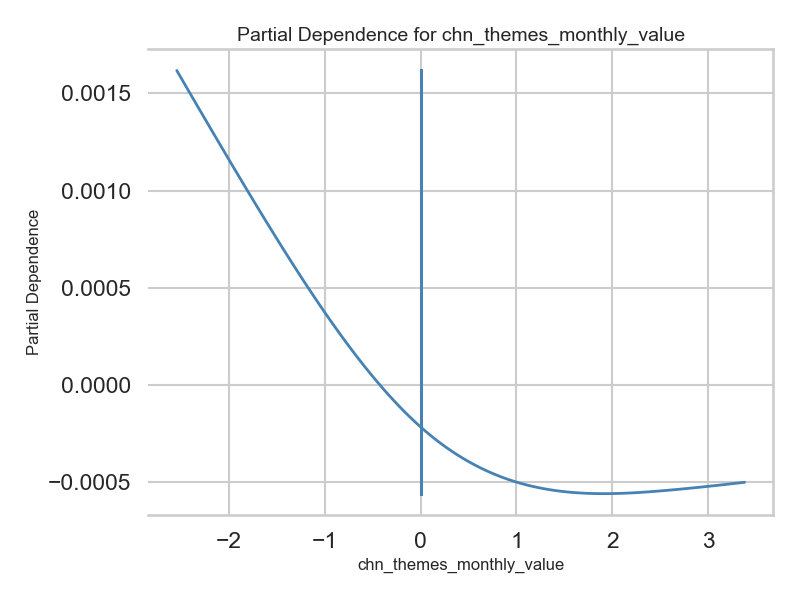
\includegraphics[width=3.5in]{figures/SpAM/us/partial_chn_themes_monthly_value.png}
\caption{Partial Dependence of Chinese Value on U.S. SpAM Model}
\label{fig:label39}
\end{center}
\end{figure}

U.S. Momentum is expected to have a positive relationship with U.S. market returns. The model does not show such a relationship (see Figure~\ref{fig:label40}). Instead, there is a negative estimated relationship that contradicts economic interpretation. This could be a result of an issue with model specification, since SpAMs assume there is no interaction between the themes and can have erroneous estimations of the dependence. Still, there are cases in which a partially negative relationship can make sense, such as in cases of high returns reverting to the mean or in cases where the general market trend is negative. 

\begin{figure}[htbp]
\begin{center}
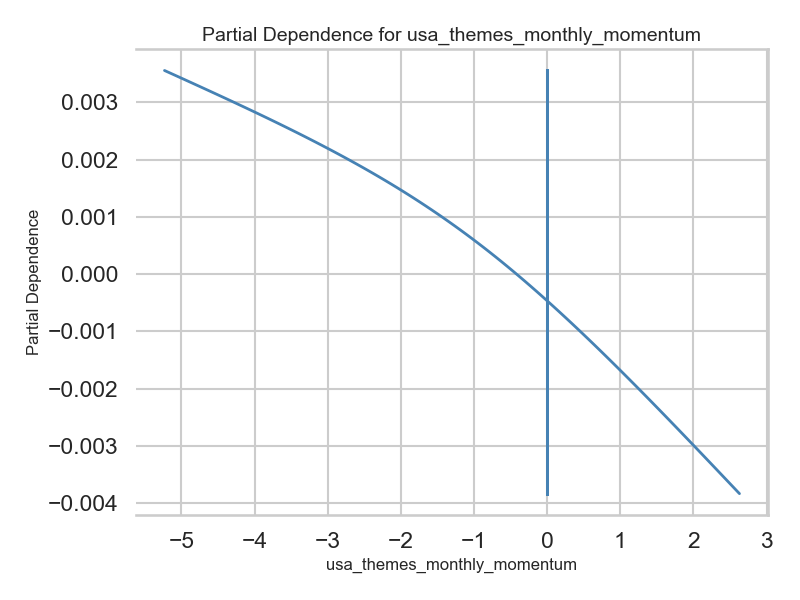
\includegraphics[width=3.5in]{figures/SpAM/us/partial_usa_themes_monthly_momentum.png}
\caption{Partial Dependence of U.S. Momentum on U.S. SpAM Model}
\label{fig:label40}
\end{center}
\end{figure}

Looking at the SpAMs for Chinese market returns, we see that the same model that overfit the U.S. market has an $R^2=0.9999$, which is likely also overfit. Generally, we see less variation in Chinese market returns being explained by the theme data, with $R^2<0.50$ across all models. The best fitting model has $R^2=0.4968$ and uses both themes and is trained on 2001 to 2024. Interestingly, we've seen this trend both times; it seems that introducing more data in these cases is far more valuable than segmenting the data due to detected structural breaks.

\begin{table}[htbp]
\centering
\caption{SpAM Regressions Predicting Chinese Market Returns}
\label{tab:spam_chn_market}
\begin{tabular}{@{}llllrr@{}}
\toprule
Time Period & Granularity & Predictors     & Adjusted $R^2$ & $R^2$ \\ \midrule
2001--2024  & Daily       & both\_themes   & 0.4357          & 0.4421 \\
2001--2024  & Daily       & chn\_themes    & 0.4278          & 0.4324 \\
2001--2024  & Daily       & usa\_themes    & 0.0173          & 0.0212 \\
2016--2024  & Daily       & both\_themes   & 0.3906          & 0.4038 \\
2016--2024  & Daily       & chn\_themes    & 0.3678          & 0.3763 \\
2016--2024  & Daily       & usa\_themes    & 0.0502          & 0.0618 \\
2001--2024  & Monthly     & both\_themes   & 0.4090          & 0.4968 \\
2001--2024  & Monthly     & chn\_themes    & 0.3903          & 0.4564 \\
2001--2024  & Monthly     & usa\_themes    & 0.0553          & 0.1055 \\
2016--2024  & Monthly     & both\_themes   & 0          & 0.9999 \\
2016--2024  & Monthly     & chn\_themes    & 0.0036          & 0.0053 \\
2016--2024  & Monthly     & usa\_themes    & 0.0752          & 0.1173 \\ \bottomrule
\end{tabular}
\end{table}

The Chinese model shows many more curves in the factors. In particular, we will examine Chinese Accruals, U.S. Profit Growth, and Chinese Momentum. Recall that the Accruals theme measures the difference between a company's reported earnings and its cash flows; lower values signal healthier earnings. 

Chinese Accruals (see Figure~\ref{fig:label41}) have a negative relationship with the Chinese market. This matches our economic intuition. Interestingly, it seems as though the theme has increasing effects as the value increases; this matches our intuition of investors detecting signals and market behavior. 

\begin{figure}[htbp]
\begin{center}
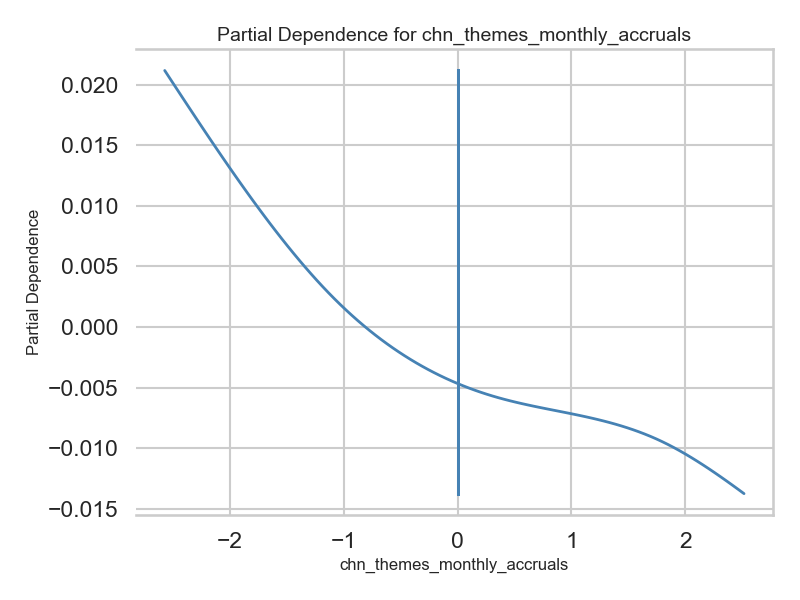
\includegraphics[width=3.5in]{figures/SpAM/china/partial_chn_themes_monthly_accruals.png}
\caption{Partial Dependence of Chinese Accruals on Chinese SpAM Model}
\label{fig:label41}
\end{center}
\end{figure}

U.S. Profit Growth (see Figure~\ref{fig:label42}) also has a negative relationship with the Chinese market. Larger values of negative profit growth in the U.S. is related to increasing Chinese market returns; this likely is a result of investors diversifying their portfolios into the Chinese market. Even more interestingly, even at 0, the partial dependence of U.S. profit growth has a negative effect on the Chinese returns. 

\begin{figure}[htbp]
\begin{center}
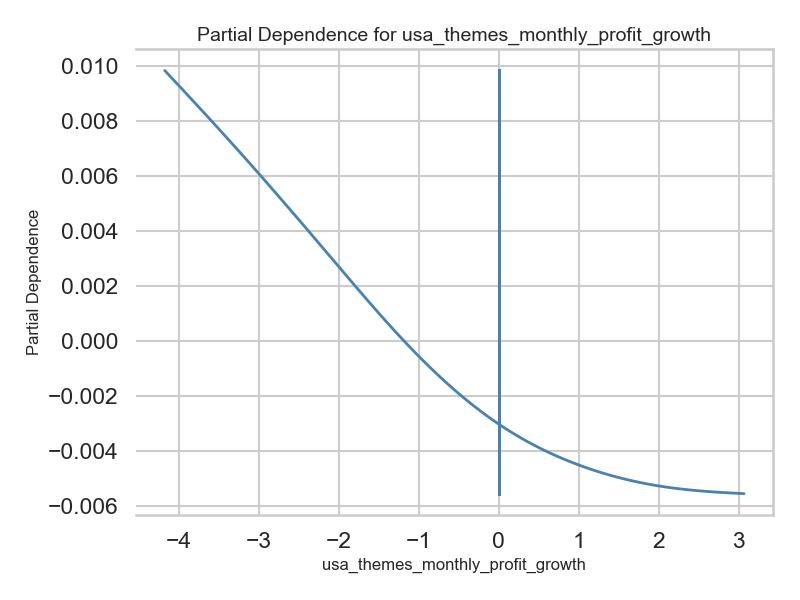
\includegraphics[width=3.5in]{figures/SpAM/china/partial_usa_themes_monthly_profit_growth.png}
\caption{Partial Dependence of U.S. Profit Growth on Chinese SpAM Model}
\label{fig:label42}
\end{center}
\end{figure}

Chinese Momentum (see Figure~\ref{fig:label43}) also has a negative relationship with the Chinese market. This is interesting as the previous SpAM model also detected such a relationship. While this doesn't match basic economic intuition, it poses an interesting trend in the data. 

I also ran 24 other SpAMs on the factor data (see Table~\ref{tab:spam_factors_summary_daily} for results). The monthly data with the factors all overfit to the data, showing an $R^2=1$ and having more factors than observations in the dataset. Similar trends occurred in cases where daily data was used for the 2016-2024 time period. Of the models that used the 2001-2024 data at a daily granularity, the U.S. factors had an $R^2=0.7900$ on the U.S. market and the Chinese factors had an $R^2=0.6021$ on the Chinese market. The results for the 2001-2024 models using the daily data are also shown in Table~\ref{tab:spam_factors_summary_daily_full}.

\begin{table}[htbp]
\centering
\caption{2021-2024 Factor-Based SpAM Regression Summary}
\label{tab:spam_factors_summary_daily_full}
\begin{tabular}{@{}lllllrrr@{}}
\toprule
Time Period & Granularity & Target Market & Predictors     & Adjusted $R^2$ & $R^2$ \\ \midrule
2001--2024  & Daily       & USA           & usa\_factors   & 0.7768         & 0.7900 \\
2001--2024  & Daily       & USA           & chn\_factors   & 0.0216         & 0.0565 \\
2001--2024  & Daily       & USA           & both\_factors  & 0.7606         & 0.7767 \\
2001--2024  & Daily       & China         & usa\_factors   & 0.0564         & 0.0871 \\
2001--2024  & Daily       & China         & chn\_factors   & 0.5815         & 0.6021 \\
2001--2024  & Daily       & China         & both\_factors  & 0.5874         & 0.6152 \\ \bottomrule
\end{tabular}
\end{table}

The SpAM models we've fit have shown nonlinear relationships among the predictors, but they assume an additive relationship and do not account for interactions between the terms. Kernel regressions are explored next as a nonparametric way to explore the dependencies between themes and market returns.

\section{Kernel Regression}

Kernel regression assumes nothing about the form of the relationship between the predictors and the outcomes, making it the most flexible of all models used so far.

Using statsmodels' KernelReg with a Gaussian kernel and the Nadaraya-Watson estimator, I fit 24 kernel regressions total on the U.S. and Chinese markets using only the themes data. The themes data was chosen to increase interpretability of the model. Of the 24 models, all 12 using data at the monthly granularity overfit (see Table~\ref{tab:kernel_overfit}). Of the 6 models assigned to each countries' returns, 2 only include the U.S. themes, 2 only include the China themes, and 2 include both. The results of the models are shown in Table~\ref{tab:kernel_regression_summary}.

\begin{table}[htbp]
\centering
\caption{Kernel Regression Summary}
\label{tab:kernel_regression_summary}
\begin{tabular}{@{}llllrr@{}}
\toprule
Time Period & Market & Data Used  & \# Predictors   & Adjusted $R^2$ & $R^2$ \\ \midrule
2001--2024    & China         & both\_themes & 26 & 0.9836         & 0.9837 \\
2001--2024    & China         & chn\_themes  & 13  & 0.9041         & 0.9043 \\
2001--2024    & China         & usa\_themes  & 13  & 0.1101         & 0.1122 \\
2001--2024  & USA           & both\_themes  & 26 & 0.9913         & 0.9914 \\
2001--2024   & USA           & chn\_themes  & 13  & -0.0024        & 4.6e-15 \\
2001--2024    & USA           & usa\_themes  & 13  & 0.8821         & 0.8824 \\
2016--2024    & China         & both\_themes & 38  & 0.9992         & 0.9992 \\
2016--2024    & China         & chn\_themes  & 15  & 0.8505         & 0.8516 \\
2016--2024   & China         & usa\_themes  & 23  & 0.9056         & 0.9067 \\
2016--2024    & USA           & both\_themes & 38  & 0.9998         & 0.9998 \\
2016--2024     & USA           & chn\_themes  & 15  & 0.7900         & 0.7916 \\
2016--2024    & USA           & usa\_themes   & 23 & 0.9523         & 0.9529 \\ \bottomrule
\end{tabular}
\end{table}

Recall that the bandwidth, which represents the length of the boundary by which points are designated as neighboring, is a very important hyperparameter in kernel regressions. A very small bandwidth causes the model to overfit and a very large bandwidth causes the model to underfit. To decrease the search space for datasets at the daily granularity, bandwidth selection was done by randomly choosing 25\% of the data and using that subsample to determine the optimal bandwidth using cross validation. This is likely why the fifth model in Table~\ref{tab:kernel_regression_summary} has such a low $R^2$. The $R^2$ would have likely been low as we've seen that Chinese themes very weakly explain the variability in U.S. returns and do so at a weaker trend than the vice versa, which had an $R^2=0.1122$.

Analyzing plots that show the predicted and actual results of each model, we draw important insights on how the models performed with the different information they were provided.

Looking at the kernel regressions fit on the Chinese market returns first, we see that the model was able to reproduce some of the general trends in the data using the Chinese themes only (see Figure~\ref{fig:labelchn1}). The model that used both the U.S. and Chinese themes performed even better, picking up on better trends in the data and making more accurate predictions (see Figure~\ref{fig:labelchn2}). This shows that there are some signals being picked up by the data, though their estimated functions might be overfit.

\begin{figure}[htbp]
\begin{center}
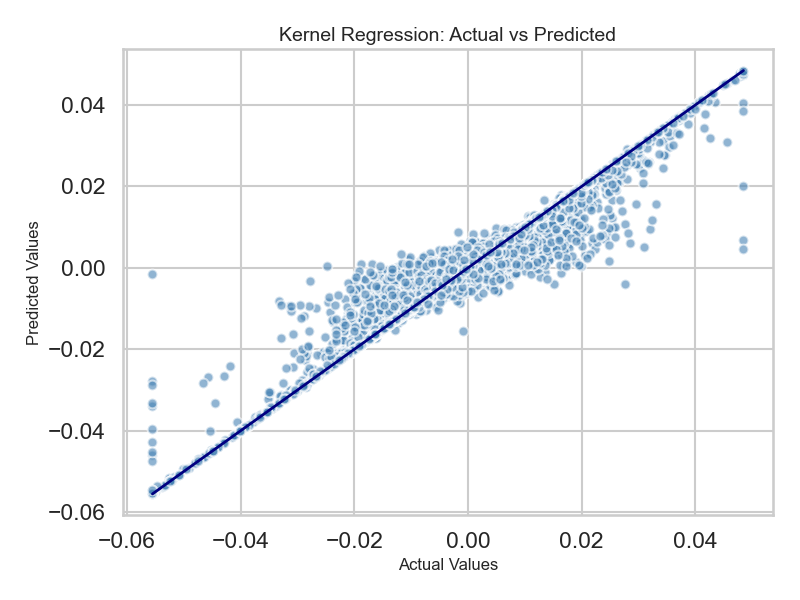
\includegraphics[width=3.5in]{figures/kernel/daily_themes_full_chn_market_daily_market_value_chn_themes_kernel.png}
\caption{Chinese Market Kernel Regression (Chinese Themes): Actual vs Predicted}
\label{fig:labelchn1}
\end{center}
\end{figure}

\begin{figure}[htbp]
\begin{center}
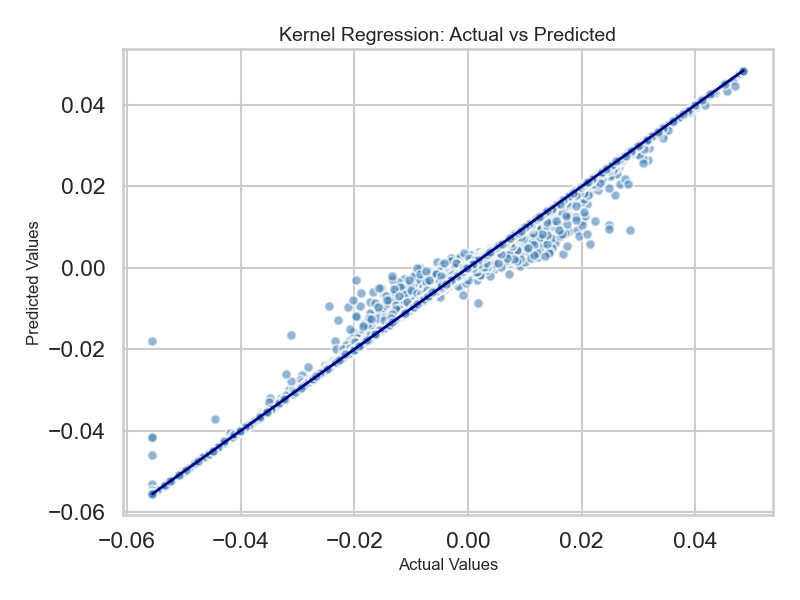
\includegraphics[width=3.5in]{figures/kernel/daily_themes_full_chn_market_daily_market_value_both_themes_kernel.png}
\caption{Chinese Market Kernel Regression (Chinese and U.S. Themes): Actual vs Predicted}
\label{fig:labelchn2}
\end{center}
\end{figure}

Most interesting is the kernel regression on the Chinese market that uses only U.S. themes, shown in Figure~\ref{fig:labelchn3}. Even with the economic themes from the U.S., the model frequently predicted values very close to 0, even when the actual values were quite far. We note that some of the trends are picked up by the signals; we see that points tend to be estimated somewhere between 0 and the actual value for estimates within [-0.02, 0.02].

\begin{figure}[htbp]
\begin{center}
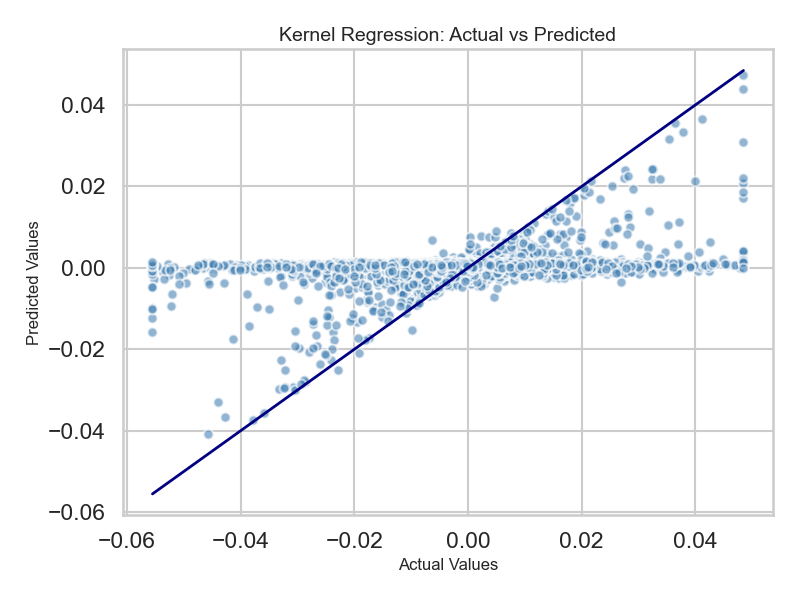
\includegraphics[width=3.5in]{figures/kernel/daily_themes_full_chn_market_daily_market_value_usa_themes_kernel.png}
\caption{Chinese Market Kernel Regression (U.S. Themes): Actual vs Predicted}
\label{fig:labelchn3}
\end{center}
\end{figure}

The U.S. market exhibited similar trends in the kernel regressions where it only had U.S. themes and themes from both countries (see Figure~\ref{fig:labelus1} and Figure~\ref{fig:labelus2}). The most interesting portion of this analysis was when looking at the kernel regression on the U.S. market that only had access to the Chinese economic themes. The model consistently predicted 0 for returns (see Figure~\ref{fig:labelus3}), indicating no signal being picked up from the Chinese themes.

\begin{figure}[htbp]
\begin{center}
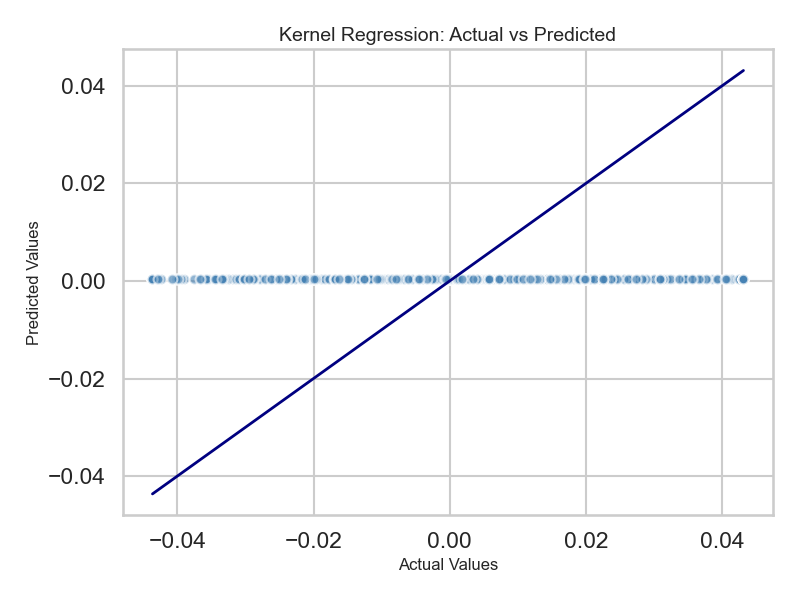
\includegraphics[width=3.5in]{figures/kernel/daily_themes_full_usa_market_daily_market_value_chn_themes_kernel.png}
\caption{U.S. Market Kernel Regression (Chinese Themes): Actual vs Predicted}
\label{fig:labelus3}
\end{center}
\end{figure}

We know this to be consistent with our other models. Generally, the Chinese market is related to changes in signals from the U.S. economy at a rate much higher than the U.S. market's equivalent with the Chinese economy. 

Analyzing the Chinese kernel model that used both Chinese and U.S. economic themes over the 2001 to 2024 time period, we notice a case of potentially conflicting signals being picked up from the U.S. market from profitability and profit growth, several curves that do not align with economic intuition, and other curves that do align with economic intuition. 

Of the curves that do match economic intuition, we notice a few trends that have opposite directions in the data. Chinese value has a positive linear relationship with the Chinese returns, shown in Figure~\ref{fig:kernelregex1}. An opposite reaction is shown in the U.S. value, which is negative relationship with Chinese returns, shown in Figure~\ref{fig:kernelregex2}. These match our economic intuition. The Chinese market returns should increase when Chinese companies have more value and decrease when U.S. companies have more value.

The partial dependence plots for U.S. profit growth and profitability were also conflicting. Chinese market returns had a smooth negative relationship with U.S. profitability (see Figure~\ref{fig:kernelregex4}), which matches our economic intuition. However, the relationship with U.S. profit growth is seen as a generally positive one, with a negative effect in [-2, 1] (see Figure~\ref{fig:kernelregex3}). Although this seems to be potentially conflicting information, it does not go against our economic intuition. Cases in which U.S. companies are either experiencing tremendous change can be caused by significant global situations that impact both countries.  

\begin{figure}[htbp]
\begin{center}
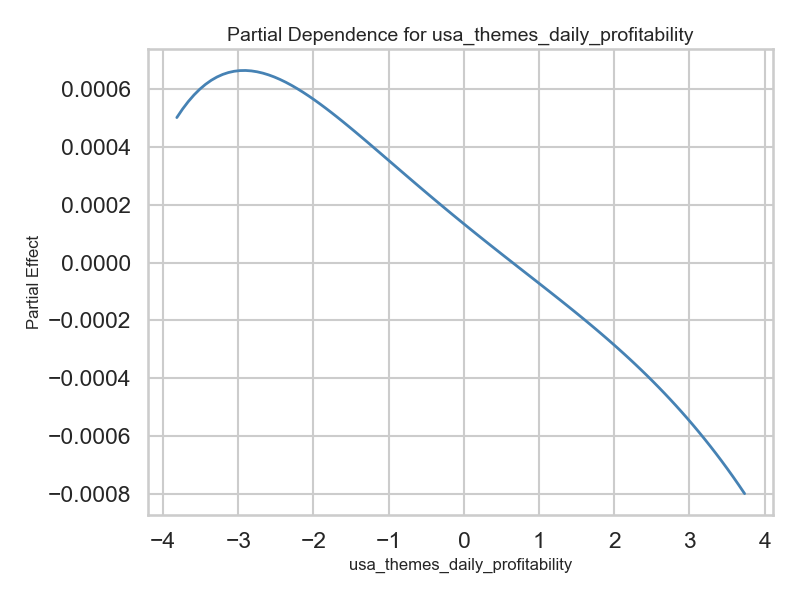
\includegraphics[width=3.5in]{figures/kernel/example/partial_effect_usa_themes_daily_profitability.png}
\caption{Partial Dependence for Chinese Kernel Regression: U.S. Profitability}
\label{fig:kernelregex4}
\end{center}
\end{figure}


\begin{figure}[htbp]
\begin{center}
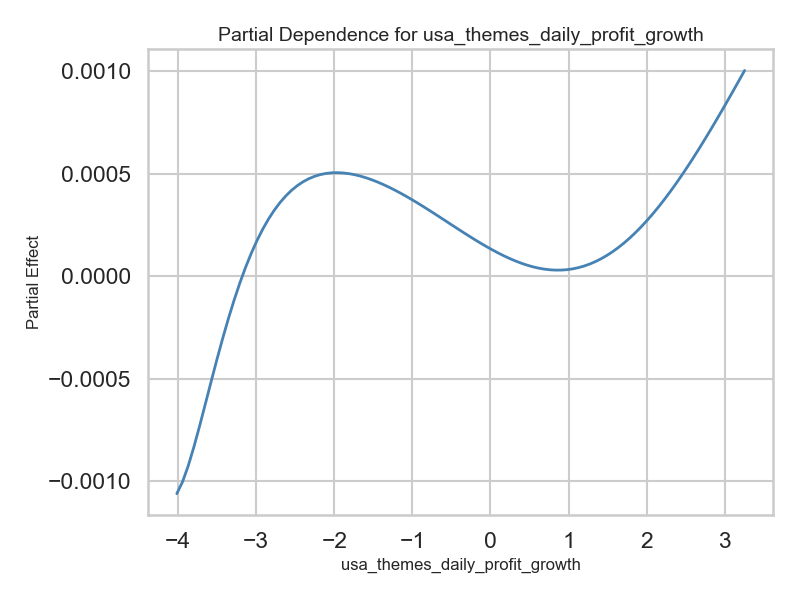
\includegraphics[width=3.5in]{figures/kernel/example/partial_effect_usa_themes_daily_profit_growth.png}
\caption{Partial Dependence for Chinese Kernel Regression: U.S. Profit Growth}
\label{fig:kernelregex3}
\end{center}
\end{figure}

There were also two cases of potential overfitting. The U.S. Accruals and U.S. Low Leverage Growth showed rocky curves with un-intuitive trends towards the extremes of the data, see Figure ~\ref{fig:kernelregex5} and Figure ~\ref{fig:kernelregex6}. 

\begin{figure}[htbp]
\begin{center}
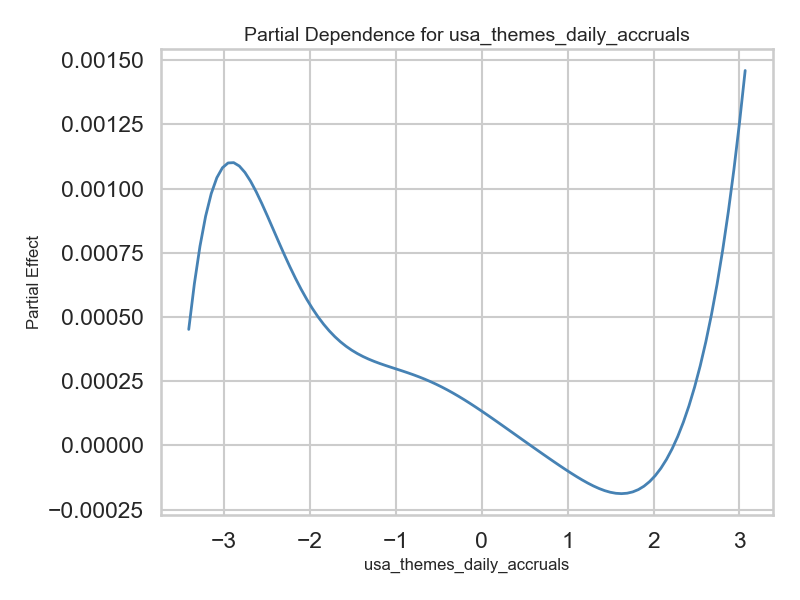
\includegraphics[width=3.5in]{figures/kernel/example/partial_effect_usa_themes_daily_accruals.png}
\caption{Partial Dependence for Chinese Kernel Regression: U.S. Accruals}
\label{fig:kernelregex5}
\end{center}
\end{figure}